%%%%%%%%%%%%%%%%%%%%%%%%%%%%%%%%%%%%%%%%%%%%%%%%%%%%%%%%%%%%%%%%%%%%%%%%%%%%%%%
% SECTION 12.1: Introduction - Willingness to Act
% Module: BCM2_06_WAX_7250
% EBF Questions: 1 (τ) and 4 (WAX, θ)
%%%%%%%%%%%%%%%%%%%%%%%%%%%%%%%%%%%%%%%%%%%%%%%%%%%%%%%%%%%%%%%%%%%%%%%%%%%%%%%

%------------------------------------------------------------------------------
% DIE 9 FRAGEN NAVIGATION BOX
%------------------------------------------------------------------------------

\begin{tcolorbox}[
  title={\textbf{Die 9 Fragen des EBF — Kapitelnavigation}},
  colback=blue!3,
  colframe=blue!50!black,
  fonttitle=\bfseries\sffamily,
  coltitle=white,
  boxrule=0.8pt,
  arc=2mm
]
\small\sffamily
\begin{tabular}{@{}clr@{}}
$\checkmark$ & 0. Kontext und Zielverhalten definieren & [Kapitel 6] \\
$\checkmark$ & 2. WELCHEN NUTZEN bringt das Verhalten? & [Kapitel 10] \\
$\checkmark$ & 3. WIE NIMMT er/sie den Nutzen WAHR? & [Kapitel 11] \\[3pt]
\rowcolor{blue!10}
$\rightarrow$ & \textbf{1. WIE denkt er/sie? (Thinking Style $\tau$)} & \textbf{[DIESES KAPITEL]} \\
\rowcolor{blue!10}
$\rightarrow$ & \textbf{4. WIE GROSS ist WAX? WELCHE SCHWELLEN $\theta$?} & \textbf{[DIESES KAPITEL]} \\[3pt]
$\circ$ & 5. WO in der Behavioral Change Journey? & [Kapitel 13] \\
$\circ$ & 6. WELCHES Behavioral Change Segment? & [Kapitel 14] \\
$\circ$ & 7. WILLINGNESS TO EFFECTIVELY CHANGE? & [Kapitel 15] \\
$\circ$ & 8. EFFEKTIVE WAHRSCHEINLICHKEIT P(Handlung)? & [Kapitel 16] \\
\end{tabular}
\end{tcolorbox}

\section{Willingness to Act: The Action Condition}
\label{sec:willingness-intro}

Chapter~\ref{ch:awareness} established \\textbf{Awareness} (AWX) — what people perceive 
of the potential utility. But perception alone does not guarantee action. 
This chapter addresses the next critical condition: \textbf{Willingness to Act} (WAX).

\begin{note}[Formal Foundation]
The complete formal specification of all Willingness axioms (99+) is provided in 
\textbf{Appendix~\ref{app:willingness-formalization}} (Willingness Formalization). 
Each axiom is documented across eight dimensions: ID, Title, Definition, 
Formal Logic, $\Psi$-Sensitivity, Empirical Reference, Testable Prediction, 
and Intervention Lever.
\end{note}

%------------------------------------------------------------------------------
\subsection{From Awareness to Willingness}
\label{subsec:12-1-from-awareness}
%------------------------------------------------------------------------------

\begin{intuition}
\textbf{The Gap Between Knowing and Doing}

Consider the difference:
\begin{itemize}
\item \textbf{Awareness} answers: ``Do I \textit{see} the benefits?''
\item \textbf{Willingness} answers: ``Am I \textit{ready} to act on them?''
\end{itemize}

A person can be fully aware of the benefits of exercise but still unwilling 
to go to the gym. A smoker may know exactly what cigarettes do to their lungs 
but remain unwilling to quit. The gap between knowing and doing is precisely 
where Willingness operates.
\end{intuition}

The relationship is sequential:

\begin{center}
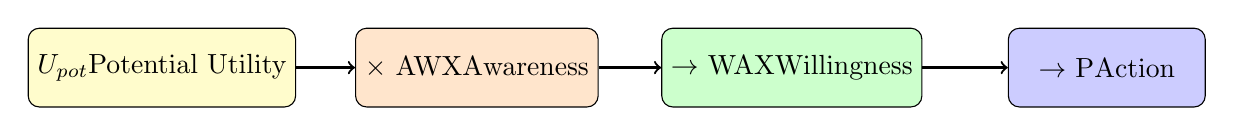
\begin{tikzpicture}[node distance=2.5cm, auto]
  \node[draw, rounded corners, fill=yellow!20, minimum width=2.5cm, minimum height=1cm] (U) {$U_{pot}$\\Potential Utility};
  \node[draw, rounded corners, fill=orange!20, minimum width=2.5cm, minimum height=1cm, right of=U, xshift=1.5cm] (AWX) {$\times$ AWX\\Awareness};
  \node[draw, rounded corners, fill=green!20, minimum width=2.5cm, minimum height=1cm, right of=AWX, xshift=1.5cm] (WAX) {$\to$ WAX\\Willingness};
  \node[draw, rounded corners, fill=blue!20, minimum width=2.5cm, minimum height=1cm, right of=WAX, xshift=1.5cm] (P) {$\to$ P\\Action};
  
  \draw[->, thick] (U) -- (AWX);
  \draw[->, thick] (AWX) -- (WAX);
  \draw[->, thick] (WAX) -- (P);
\end{tikzpicture}
\end{center}

%------------------------------------------------------------------------------
\subsection{Definition: The Willingness Function}
\label{subsec:12-1-definition}
%------------------------------------------------------------------------------

\begin{definition}[Willingness to Act -- Content]
\label{def:willingness-content}
\textbf{Willingness to Act (WAX)} is the degree to which an individual is 
prepared to execute a behavior, given their awareness of its consequences. 
WAX integrates three components:
\begin{enumerate}
\item How the person \textit{thinks} about multi-dimensional decisions (thinking style $\tau$)
\item The perceived utilities across all dimensions ($U^* = AWX \cdot U$)
\item The barriers and facilitators in the decision context
\end{enumerate}
\end{definition}

\begin{definition}[Willingness to Act -- Function]
\label{def:willingness-function}
\textbf{Willingness to Act} is the sufficient condition for action when 
it exceeds the behavioral threshold $\theta$ at the Moment of Truth ($t^*$).
\end{definition}

\paragraph{The Core Decision Formula.}
\begin{equation}
\boxed{P(\text{Action}) > 50\% \quad \Leftrightarrow \quad WAX > \theta}
\label{eq:willingness-threshold}
\end{equation}

\begin{intuition}
\textbf{In Plain Language:}

Action occurs when \textit{wanting} exceeds \textit{difficulty}:
\begin{itemize}
\item $WAX$: How much do I want this? (Willingness)
\item $\theta$: How hard is it to do? (Threshold)
\item If $WAX > \theta$: I'll probably do it
\item If $WAX < \theta$: I'll probably not do it
\end{itemize}
\end{intuition}

%------------------------------------------------------------------------------
\subsection{Two Questions, One Chapter}
\label{subsec:12-1-two-questions}
%------------------------------------------------------------------------------

This chapter answers two of the nine EBF questions:

\begin{tcolorbox}[
  colback=white,
  colframe=blue!50!black,
  title={\textbf{Questions Addressed in This Chapter}},
  fonttitle=\bfseries\sffamily
]

\textbf{Question 1: How does the person think? ($\tau$)}

The \textbf{Thinking Style Parameter} $\tau \in [0,1]$ captures whether 
a person integrates multiple utility dimensions in a connected (complementary) 
or separated (additive) way:

\begin{center}
\begin{tabular}{lp{8cm}}
$\tau \to 1$ & ``Everything must be right'' — weakest dimension dominates\\
$\tau \to 0$ & ``Total benefit counts'' — dimensions add up\\
\end{tabular}
\end{center}

\vspace{6pt}
\textbf{Question 4: How large is WAX? What are the thresholds $\theta$?}

The \textbf{Willingness to Act} combines thinking style and effective utilities:
\begin{equation*}
WAX = \tau \cdot \min\{U^*\} + (1-\tau) \cdot \sum U^*
\end{equation*}

The \textbf{Behavioral Threshold} depends on decision type and context:
\begin{equation*}
\theta = \theta_{base}(d) + \sum_j \delta_j \cdot \Psi_j
\end{equation*}

\end{tcolorbox}

%------------------------------------------------------------------------------
\subsection{Chapter Structure}
\label{subsec:12-1-structure}
%------------------------------------------------------------------------------

This chapter proceeds as follows:

\begin{itemize}
\item \textbf{Section 12.2}: The Thinking Style Parameter $\tau$ — How people integrate multiple dimensions
\item \textbf{Section 12.3}: The WAX Formula — Calculating Willingness to Act
\item \textbf{Section 12.4}: The Threshold $\theta$ — What determines how hard a decision is
\item \textbf{Section 12.5}: The Critical Comparison — WAX vs. $\theta$ and the three regimes
\item \textbf{Section 12.6}: Complete Example — Anna's journey from 34\% to 54\%
\item \textbf{Section 12.7}: Axiom Overview — The formal foundation in Appendix UNMAPPED_REA
\item \textbf{Section 12.8}: $\Psi$-Context Modulation — How context shifts both WAX and $\theta$
\item \textbf{Section 12.9}: Summary — Key formulas and connection to Chapters 13--16
\end{itemize}

\begin{cross-reference}
\textbf{Formal Specification:} For complete mathematical formalization including 
all 99+ axioms, the $\gamma$-matrix for $\tau$-estimation, the $\delta$-matrix 
for threshold modulation, and the 8-factor documentation framework, 
see \textbf{Appendix UNMAPPED_REA} (Willingness Formalization).
\end{cross-reference}

